\documentclass[oneside,pwrcover,withmarginpar,hidelinks,11pt]{article}
%\documentclass[twoside,11pt]{report}

\sloppy
\usepackage{url}
\usepackage{algorithm}
\usepackage{algorithmic}
\usepackage{covington} % numbered examples
\usepackage{color} % TODOs
\usepackage[table]{xcolor}
\usepackage{adjustbox}
\usepackage{enumitem}

\usepackage[backend=bibtex,defernumbers=true]{biblatex}
\addbibresource[label=pwr]{./bib/pwr-wlasne}

\usepackage{amsmath, amsthm, amssymb,amsfonts}

\usepackage{verbatim}
\usepackage{graphicx}


\usepackage{colortbl}
\definecolor{violet}{rgb}{.4,.1,.8}
\newcommand\map[1]{{\footnotesize \fontfamily{phv}\selectfont \textcolor{blue}{#1}}}

\newcommand{\todo}[1]{\textcolor{red}{{\bfseries TODO:} #1}}

\usepackage[polish]{babel}
\usepackage[T1]{fontenc}
\usepackage[utf8]{inputenc}
\usepackage{bussproofs}
\usepackage{cmll}
\newcommand{\tensor}{\bullet}
\newcommand{\forward}{\operatorname{/}}
\newcommand{\backward}{\operatorname{\backslash}}
\newcommand{\both}{\mid}
\newcommand{\plus}{\oplus}
\newcommand{\maybe}{?}
\newcommand{\zero}{0}
\newcommand{\one}{1}

\title{Kategorialny Parser Składniowo-Semantyczny „ENIAM”\\{\Large dokumentacja techniczna}}
\author{Wojciech Jaworski}
%\date{}

\begin{document}

\maketitle
 
\section{Ogólny opis}

Kategorialny Parser Składniowo-Semantyczny „ENIAM” jest narzędziem generującym {\it formy logiczne/reprezentacje semantyczne} dla zdań w języku polskim. 
Parser pracuje na niepreparowanych danych, realizuje kolejne etapy przetwarzania tekstu: tokenizację, 
lematyzację, rozpoznawanie związków składniowych, anotację sensami słów oraz rolami tematycznymi, 
częściową dezambiguację oraz tworzenie reprezentacji semantycznej.

Poniższy dokument opisuje w jaki sposób zaimplementowane są poszczególne komponenty parsera.


\section{Preprocessing}

Kolejne etapy przetwarzania tekstu realizowane są w ramach rozmytego potoku przetwarzania.
Parser nie dezambiguuje na bieżąco niejednoznaczności powstającej po każdym kroku przetwarzania tekstu.
Zamiast tego tworzy zwartą reprezentację niejednoznacznego wyniku, którą przekazuję do następnego etapu,
dezambiguację wykonuje pod koniec potoku przetwarzania.

Podejście to jest uzasadnione spostrzeżeniem, że 
dezambiguacja działa poprawnie jedynie w pewnym procencie przypadków,
a złożenie kilku procedur, które nie działają całkowicie poprawnie radykalnie zmniejsza szansę uzyskania poprawnego wyniku.
Np. tagery dla języka polskiego mają skuteczność ok 93\%, w zdaniu występuje średnio 15 słów, 
więc prawdopodobieństwo poprawnego otagowania typowego zdania wynosi $0,93^{15}=0,3367$.

Początkowe etapy przetwarzania tekstu (poprzedzające określenie struktury zależnościowej)
będziemy określać mianem preprocesingu. Etapy te realizowane są przez program {\tt pre} stanowiący
wolnostojący serwer sieciowy, z którym komunikuje się parser {\tt eniam}.

Podczas preprocesingu tekst reprezentowany jest jako graf, 
którego krawędzie etykietowane są tokenami.
Do takiego grafu dodawane są i usuwane nowe krawędzie i wierzchołki.
Przykładowy graf:
\begin{center}
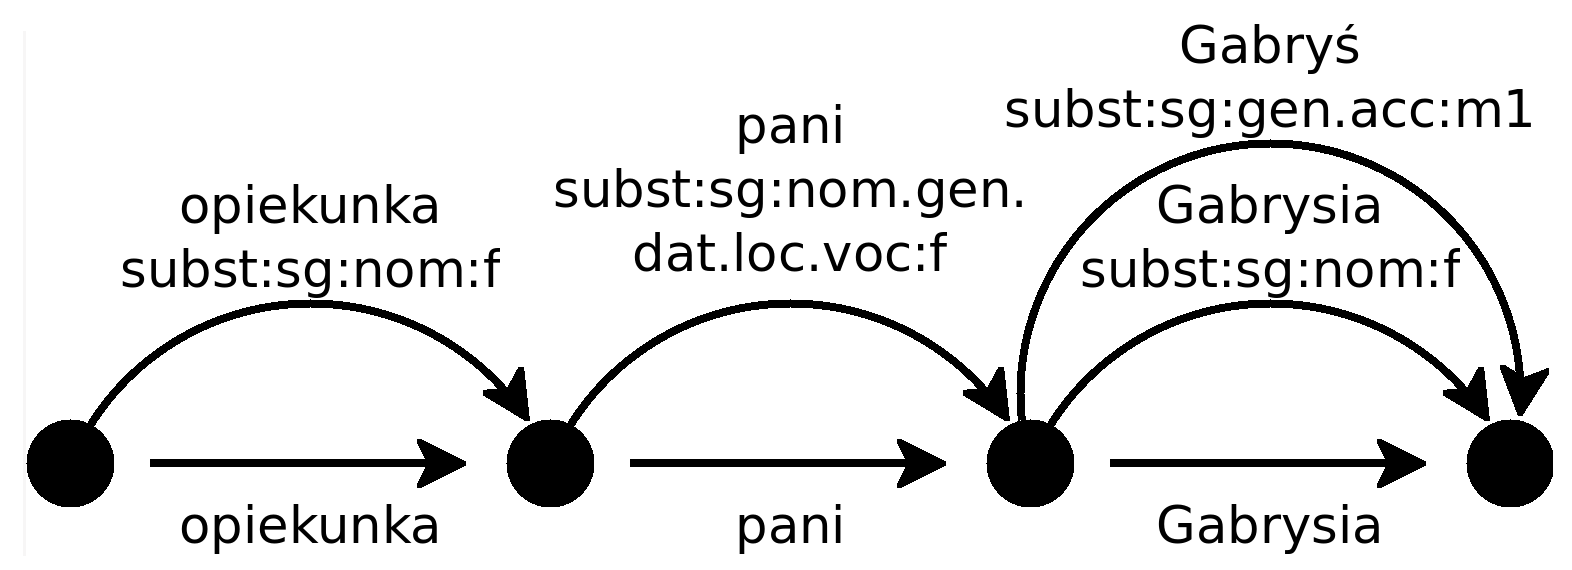
\includegraphics[width=12cm]{opiekunka.png}
\end{center}

Podczas preprocesingu następuje integracja zasobów.
Przetwarzane zdanie anotowane jest m. in. informacjami 
pochodzącymi następujących zasobów: SGJP, Słowosieć, Walenty. %Polimorf, 
Kolejne etapy preprocesingu to tokenizacja, lematyzacja, wykrywanie nazw własnych, określanie sensów słów, określanie walencji.

\subsection{Tokenizacja}
Przed właściwą tokenizacją następuje podział tekstu na znaki, 
klasyfikacja znaków na litery wielkie, litery małe, cyfry, symbole i pozostałe znaki.
Literom wielkim przyporządkowywane są ich małe odpowiedniki.
Analizowane są następujące bloki Unicode: Basic Latin, Latin-1 Supplement, Latin Extended-A, Latin Extended-B, Latin Extended Additional, General Punctuation, Currency Symbols.

Następnie ma miejsce łączenie znaków w tokeny. Tokeny należą do następujących typów:
\begin{itemize}
\item sekwencje cyfr wraz z typami np: liczby naturalne, sekwencje 3-cyfrowe, numery miesięcy
\item liczby rzymskie wraz z tłumaczeniem na arabskie
\item sekwencje liter z podziałem na sekwencje małych liter, sekwencje wielkich, 
sekwencje małych poprzedzone wielką i inne.
\item symbole,
\item proste i złożone znaki interpunkcyjne,
\item emotikony.
\end{itemize}
Różnica pomiędzy symbolem a znakiem interpunkcyjnym polega na tym, że 
symbole są elementami złożonych tokenów, a znaki interpunkcyjne uczestniczą w analizie składniowej.

W ramach sekwencji liter następuje interpretacja użycia wielkich liter.
Jeśli sekwencja zaczyna się od wielkiej litery może należeć do jednej z trzech kategorii:
może być nazwą własną, być początkiem zdania lub nazwą własną na początku zdania.
Jeśli sekwencja składa się z samych wielkich liter może być 
napisana tak z przyczyn stylistycznych lub być akronimem --- 
zapis nie wskazuje wtedy czy jest to nazwa własna lub początek zdania.
Rozpoznawane są też sufiksy: -em, -m, -eś, -ś, -eśmy, -śmy, -eście, -ście, -by, -że, -ż i traktowane jako odrębne tokeny.

Podczas tokenizacji symboli następuje ujednolicenie symboli używanych do zapisania znaków interpunkcyjnych takich jak
spacje, cudzysłowy, apostrofy, myślniki czy dywizy.
Przykładowo znak '\"' interpretowany jest jako cudzysłów otwierający '„' lub cudzysłów zamykający '”',
dwa następujące po sobie przecinki ',,' interpretowane są jako cudzysłów otwierający,
a dwa następujące po sobie apostrofy interpretowane są jako cudzysłów zamykający.

Haplologia kropki obsługiwana jest poprzez przypisanie temu symbolowi trzech 
możliwych interpretacji: tokenu końca zdania, tokenu symbolu (np. elementu skótu), tokenu końca zdania poprzedzonego tokenem symbolu.
Podobnie rozwiązywana jest haplologia wielokropka.
Przykładowo kropka fragment w poniższym tekstu 
\begin{center}
{\it \dots w XV w. Warszawa \dots}, 
\end{center}
może w połączeniu z poprzedzającą literą 'w' stanowić skrót formy 'wieku', a niezależnie od tego może stanowić koniec zdania. 
Jeśli kropka ta oznacza koniec zdania, wielka liter w formie 'Warszawa' może oznaczać początek zdania i nazwę własną,
lub jedynie początek zdania.

Przecinek interpretowany jest jako początek i koniec zdania składowego, symbol (np. element notacji dziesiętnej), 
znak interpunkcyjny oznaczający koordynację.

Kolejnym krokiem jest rozpoznawanie złożonych tokenów
obejmujące liczby %(NKJP1M):
\begin{center}
pref3dig . 3dig . 3dig . 3dig $\to$ natnum\\
day . month . year $\to$ date\\
- natnum , dig $\to$ realnum
\end{center}
odmienione akronimy i nazwiska obce %(SGJP i Polimorf): %TODO: złączyć reguły, uzupełnić o to co jest w korpusie, dodać p-wstwa.
\begin{center}
* - ów $\to$ *:subst:pl:acc:m1|subst:pl:gen:m1.m2.m3.n2\\
* - cie $\to$ *T:subst:sg:loc.voc:m3\\
* - cie $\to$ *TA:subst:sg:dat.loc:f\\
* - owscy $\to$ *-owski:adj:pl:nom.voc:m1.p1:pos\\
* ’ ego $\to$ *:subst:sg:gen.acc:m1
\end{center}
leksemy wielotokenowe %(SGJP i Polimorf):
\begin{center}
ping - ponga $\to$ ping-pong:subst:sg:gen.acc:m2\\
rock ’ n ’ rollem $\to$ rock’n’roll:subst:sg:inst:m2
\end{center}
i skróty rozwijane do sekwencji wielu tokenów
\begin{center}
br . $\to$ bieżący:adj:sg:\$C:m3:pos rok:subst:sg:\$C:m3\\
\end{center}
Wyszukiwane są tu najdłuższe dopasowania, a 
znalezione dopasowania zastępują rozpoznane sekwencje tokenów.

%Walidacja tokenizacji została przeprowadzona na NKJP1M v.1.2 i wykazała,
%że tokenizacja ENIAM-a różni się od tokenizacji NKJP1M na 9474 tokenach,
%z czego w przypadku 782 tokenów jest to błąd tokenizacji ENIAM-a.
% 52      eniam-correct
% 707     tys.
% 782     nkjp-correct
% 7933    both-correct

%stan na 2017.10.07
Walidacja tokenizacji została przeprowadzona na NKJP1M v.1.2 i wykazała,
że tokenizacja ENIAM-a różni się od tokenizacji NKJP1M na 9462 tokenach,
z czego w przypadku 764 tokenów jest to błąd tokenizacji ENIAM-a.
55      eniam-correct
470     letni
707     tys.
764     nkjp-correct
1401    brev
6065    both-correct

\subsection{Lematyzacja}

%TODO: opisać guesser
Lematyzacja wykonywana jest na podstawie SGJP-20160724.% oraz Polimorf-20151020.
W pierwszym kroku na podstawie końcówki słowa odnajdywane są możliwe lematy i interpretacje.
W drugim kroku następuje wybór znanych lematów spośród odnalezionych.
Jeśli żaden znany lemat nie jest wystąpił wśród odnalezionych zwracane są wszystkie 
odnalezione lematy i interpretacje. %utworzone na podstawie reguł mających wysokie wsparcie w słowniku. 
Tokeny będące sekwencjami małych liter poprzedzonych wielką literą
są lematyzowane w swojej pierwotnej postaci, a w razie niepowodzenia w 
wersji ze zmniejszoną pierwszą literą.
\begin{center}
Kotem $\to$ kotem $\to$ kot subst:sg:inst:m2 $\to$ Kot subst:sg:inst:m2
\end{center}

Na tym etapie wykonywane jest też rozwijanie skrótów oraz rozpoznawanie wyrażeń wielosłownych.
%TODO: integracja z SEJFem i innymi 
%TODO: opisać jak

%TODO: opisać: heurystyka tagująca nieznane tokeny

\subsection{Nazwy własne}
Oznaczenie nazwami własnymi wykonywane jest za pomocą list 
wytworzonych na podstawie SGJP-20151020 oraz Polimorf-20151020,
uzupełnionych o inicjały, nazwy dni tygodnia i miesięcy.
Nazwom przyporządkowywane są ich typy np.: toponim, nazwisko
oraz typy obiektów wskazywanych przez nazwy np.: obszar, osoba.
Aktualnie tylko rzeczowniki mogą być nazwami własnymi.
Rzeczowniki napisane wielką literą, ale nie znalezione w słowniku
nazw własnych traktowane są jako nazwy własne nieznanego typu.
%TODO: integracja z NELexicon 2.0, Liner2

\subsection{Sensy słów}
Sensy słów przypisywane są do lematów na podstawie Słowosieci 2.1.0.
Sensy reprezentowane są jako lematy zaopatrzone w numery wariantów i 
uzupełnione są o listy hiperonimów.
Hiperonimy to synsety reprezentowane przez kanonicznie wybrane sensy.
%\item Aktualnie nie korzystam z liczbowych identyfikatorów ze Słowosieci.
Nazwom własnym przypisywane są sensy wynikające z ich typów.    
Na przykład leksemowi {\it zamek} zostaną przypisane m. in. następujące sensy wraz z hiperonimami:
\begin{description}
\item{\bf zamek 1} budowla: rezultat 1, wytwór 1, konstrukcja 1, budowla 1, budynek 1, dom 1, rezydencja 1, zamek 1
\item{\bf zamek 2} urządzenie do zamykania: obiekt 2, rzecz 4, przedmiot 1, zamknięcie 12, zamek 2
\item{\bf zamek 6} suwak: obiekt 2, rzecz 4, przedmiot 1, zamknięcie 12, zapięcie 2, zamek błyskawiczny 1
\end{description}
%TODO: integracja ze Słowosiecią 3.0, uogólnienie hiponimii przez dodanie innych relacji

\subsection{Walencja leksemów}
Walencja leksemów zawartych w zdaniu ustalana jest na podstawie
słownika walencyjnego Walenty w wersji dnia 2016.04.12.
{\it Walenty} zawiera schematy opisujące cechy składniowe podrzędników wybranych czasowników, rzeczowników, przymiotników i przysłówków,
ramy opisujące cechy semantyczne (role tematyczne i preferencje selekcyjne) podrzędników,
oraz powiązania pomiędzy schematami i ramami.
Na potrzeby parsowania łączymy ramy ze schematami.

%\item Relacyjne preferencje selekcyjne na razie nie są zaimplementowane.
Przed parsowaniem następuje dezambiguacja (selekcja) hiperonimów i preferencji selekcyjnych:
pozostają tylko te hiperonimy, dla których występuje w segmencie odpowiednia preferencja selekcyjna
i tylko te preferencje selekcyjne, dla których występuje w segmencie odpowiedni hiperonim.
Predefiniowane w {\it Walenty} preferencje selekcyjne zostały dodane do relacji hiperonimii w {\it Słowocieci}.

Schematy zawarte w Walentym mają charakter ogólny opisują podrzędniki 
leksemów w sposób niezależny od ich formy gramatycznej.
Aby zastosować je w praktyce trzeba je przetworzyć tak, 
by dostosować je do formy leksemu występującej w zdaniu.
Proces ten ma w dużej mierze charakter dekompresji.

Etapy przetwarzania schematu walencyjnego zaprezentujemy na poniższym przykładzie:
\begin{center}
subj,Initiator,\{np(str),ncp(str,int)\}+\\Recipent,\{refl\}+Theme,\{prepnp(o,loc);comprepnp(na temat)\}
\end{center}
Mamy tu schemat walencyjny czasownika zawierającego podmiot realizowany jako fraza
rzeczownikowa w przypadku strukturalnym lub fraza zdaniowa pytajna z korelatem (również
w przypadku strukturalnym), partykułę {\it się} oraz argument realizowany jako 
fraza przyimkowa z przyimkiem {\it o} lub {\it na temat}.
Podmiot ma tutaj rolę semantyczną Initiator, partykułę {\it się} --- \\Recipent, fraza przyimkowa --- Theme.

Pierwszym etapem przetwarzania jest 
wstawienie do schematów realizacji fraz, podtypów atrybutów i atrybutów równoważnych.
\begin{center}
subj\{np(str),ncp(str,int[co,czemu,czy,czyj,\dots])\}+\\\{refl\}+\{prepnp(o,loc);comprepnp(na temat)\}
\end{center}
Po nim następuje uzupełnienie pozycji o informację o opcjonalności.
\begin{center}
subj,Agnt\{pro,np(str),ncp(str,int[co,czemu,czy,czyj,\dots])\}+\\Ptnt\{refl\}+Arg\{null,prepnp(o,loc);comprepnp(na temat)\}
\end{center}
Usunięcie realizacji zawierających leksemy nie występujące w zdaniu.
\begin{center}
subj,Agnt\{pro,np(str),ncp(str,int[czemu])\}+\\Ptnt\{refl\}+Arg\{null\}
\end{center}
Przetwarzanie leksykalizacji (opisane w dalszym ciągu raportu).
Ukonkretnienie schematu na podstawie klasy fleksemu i jego użycia 
(wskazanie konkretnych realizacji dla atrybutów str,part,żeby2,\dots oraz zmiana realizacji subj).
\begin{center}
subj,Agnt\{pro,np(nomagr),ncp(nomagr,int[czemu])\}+\\Ptnt\{refl\}+Arg\{null\}%,nump(nomagr)
\end{center}
Uzupełnienie schematu o modyfikatory.
\begin{center}
subj,Agnt\{pro,np(nomagr),ncp(nomagr,int[czemu])\}+\\Ptnt\{refl\}+Arg\{null\}+\{null,advp\}+\{null,prepp\}
\end{center}
Dodanie informacji o cechach semantycznych.

Przetwarzanie leksykalizacji zilustrujemy następującym przykładem:\\
balansować: \{lex(prepnp(na,loc),sg,XOR('krawędź','skraj'),atr1(\{np(gen)\}))\}
Konwersja nazw fraz na nazwy fleksemów.\\
balansować: \{lex([prep(loc),'na';subst(sg,loc),XOR('krawędź','skraj')], atr1(\{np(gen)\}))\}\\
Zamiana list fleksemów na argumenty.\\
balansować: \{lex(prep(loc),'na',ratr(\{lex(subst(sg,loc),XOR('krawędź','skraj'), atr1(\{np(gen)\}))\}))\}\\
Utworzenie schematów z leksykalizacji.\\
balansować: \{lex(1,prep(loc),'na')\}\\
lex(1,na): ratr(\{lex(2,subst(sg,loc),XOR('krawędź','skraj'))\})\\
lex(2,krawędź): atr1(\{np(gen)\})\\
lex(2,skraj): atr1(\{np(gen)\})
Rozwinięcie modyfikacji.\\
lex(1,na): \{lex(2,subst(sg,loc),XOR('krawędź','skraj'))\}\\
lex(2,krawędź): \{null;np(gen)\}\\
lex(2,skraj): \{null;np(gen)\}
Rozwinięcie list lematów.\\
lex(1,na): \{lex(2,subst(sg,loc),'krawędź')\}\\
lex(1,na): \{lex(2,subst(sg,loc),'skraj')\}

Dla leksemów nie występujących w Walentym generuję schematy typowe dla ich części mowy.
%\item Informacja o byciu nazwą własną jest zawarta w walencji.
%\item Nazwy własne mają specjalną walencję.


% {Testy}
% \begin{itemize}
% \item Test wykonany na 19957 zdaniach ze {\it Składnicy}.
% \item Czas wykonania bez kosztu komunikacji między procesami: 373.535s (0.018s na zdanie).
% \item Czas wykonania wraz z kosztem komunikacji między procesami: 393.431s (0.019s na zdanie).
% \item Poprzednia wersja preprocesingu miała szybkość 0,41-0,43s na zdanie.
% \item Czas uruchamiania preprocesingu: ok. 4 minuty.
% \item Pokrycie bez niepoświadczonych lematów i niepoświadczonych nazw własnych:
% \begin{center}
% \begin{tabular}{l|rrr}
%  & liczba & pokrycie & pokrycie \\
%  & tokenów & {\it Słowosieci} & {\it Walentego} \\
% \hline
% noun & 127851 &  0.855 & 0.226\\
% verb & 59842 &  0.917 & 0.941\\
% adj & 43121 &  0.894 & 0.353
% \end{tabular}
% \end{center}
% \end{itemize}
% % bez "notvalidated proper" i "lemma not validated"
% % noun=127851 (avg=6.406324) noun_sense=109416 (avg=5.482588, 0.855809) noun_valence=28992 (avg=1.452723, 0.226764)
% % verb=59842 (avg=2.998547) verb_sense=54895 (avg=2.750664, 0.917332) verb_valence=56323 (avg=2.822218, 0.941195)
% % adj=43121 (avg=2.160695) adj_sense=38577 (avg=1.933006, 0.894622) adj_valence=15239 (avg=0.763592, 0.353401)
% % bez "notvalidated proper" 
% % noun=162763 (avg=8.155685) noun_sense=109920 (avg=5.507842, 0.675338) noun_valence=29019 (avg=1.454076, 0.178290)
% % verb=63848 (avg=3.199278) verb_sense=54907 (avg=2.751265, 0.859964) verb_valence=56331 (avg=2.822619, 0.882267)
% % adj=66690 (avg=3.341685) adj_sense=38934 (avg=1.950894, 0.583806) adj_valence=15240 (avg=0.763642, 0.228520)
% % wszystkie
% % noun=209615 (avg=10.503332) noun_sense=109920 (avg=5.507842, 0.524390) noun_valence=29019 (avg=1.454076, 0.138440)
% % verb=77252 (avg=3.870922) verb_sense=54907 (avg=2.751265, 0.710752) verb_valence=56331 (avg=2.822619, 0.729185)
% % adj=89285 (avg=4.473869) adj_sense=38934 (avg=1.950894, 0.436064) adj_valence=15241 (avg=0.763692, 0.170701)

\section{Parsowanie}
Zaanowowany podczas preprocesingu tekst przetwarzany jest następnie przez 
parser działający w oparciu o gramatykę kategorialną.
Mają tu miejsce następujące działania:
generowane wpisu w leksykonie, określanie struktury zależnościowej, 
nadawanie walencji semantycznej, dezambiguacja, tworzenie reprezentacji semantycznej. 

\subsection{Gramatyka kategorialna (Type Logical Categorial Grammar)}
Parsowanie gramatykach kategorialnych jest dowodzeniem twierdzeń w niekomutatywnej intuicjonistycznej logice liniowej.
Można dzięki temu implementować fragmenty systemu dowodowego, uzyskując szybkie parsery i mając gwarancję poprawności.

Reguły gramatyczne to uniwersalne, niezależne od przetwarzanego języka reguły dowodzenia w logice.
Powoduje to, że gramatyka jest w pełni zleksykalizowana, 
co ułatwia to integrację z zasobami słownikowymi np. Walentym

Spójniki LCG wyrażają podstawowe zjawiska występujące w języku:
\begin{itemize}
\item $\tensor$ konkatenacja (tworzenie wektorów cech)
\item $\with$ niejednoznaczność
\item $\forward$, $\backward$, $\both$ wymaganie argumentu
\item $\plus$ polimorficzne argumenty, sumowanie typów
\item $\one$ pusty argument
\item $\maybe$ wielokrotny argument
\item $\bigwith$ parametryzowana niejednoznaczność
\item $\star$ tworzenie listy
\end{itemize}
Umożliwiają bezpośrednie wyrażenie informacji dostarczanej przez lematyzację i zawartej w Walentym.
Na przykład cechy fleksyjne leksemu {\it zielony} określone podczas lematyzacji jako
\begin{center}
adj:sg:nom.voc:m1.m2.m3:pos|adj:sg:acc:m3:pos
\end{center}
może my wyrazić w gramatyce kategorialnej następująco:
\[(\text{adj}\tensor\text{sg}\tensor(\text{nom}\with\text{voc})\tensor(\text{m1}\with\text{m2}\with\text{m3})\tensor\text{pos})\with
(\text{adj}\tensor\text{sg}\tensor\text{acc}\tensor\text{m3}\tensor\text{pos})\]

Podstawową reguła w gramatyce jest aplikacja argumentu do funktora
\begin{center}
\AxiomC{$\Gamma\vdash\psi\forward\varphi$}
\AxiomC{$\Delta\vdash\varphi$}
\RightLabel{$[\forward E]$}
\BinaryInfC{$\Gamma,\Delta\vdash\psi$}
\DisplayProof
\hspace{1cm}
\AxiomC{$\Delta\vdash\varphi$}
\AxiomC{$\Gamma\vdash\psi\backward\varphi$}
\RightLabel{$[\backward E]$}
\BinaryInfC{$\Delta,\Gamma\vdash\psi$}
\DisplayProof
\end{center}
Oto przykładowy wywód gramatyczny. Będziemy w nim korzystać z leksykonu 
\[\text{Jan}_1\vdash\text{np},\;\text{widzi}_2\vdash(\text{ip}\backward\text{np})\forward\text{np},\;\text{stół}_3\vdash\text{np},\;\text{.}_4\vdash\text{s}\backward\text{ip}\]
i otrzymamy następujące drzewo wywodu:
\begin{prooftree}
\hspace{-1cm}
\AxiomC{$\text{Jan}_1\vdash\text{np}$}
\AxiomC{$\text{widzi}_2\vdash(\text{ip}\backward\text{np})\forward\text{np}$}
\AxiomC{$\text{stół}_3\vdash\text{np}$}
\BinaryInfC{$\text{widzi}_2,\text{stół}_3\vdash\text{ip}\backward\text{np}$}
\BinaryInfC{$\text{Jan}_1,\text{widzi}_2,\text{stół}_3\vdash\text{ip}$}
\AxiomC{$\text{.}_4\vdash\text{s}\backward\text{ip}$}
\BinaryInfC{$\text{Jan}_1,\text{widzi}_2,\text{stół}_3,\text{.}_4\vdash\text{s}$}
\end{prooftree}


Izomorfizm Curriego-Howarda wiąże reguły wnioskowania z termami liniowego rachunku lambda 
zadając sposób konstruowania formuł języka reprezentacji znaczenia podczas parsowania.
% zamiast występującej w innych formalizmach gramatycznych unifikacji, dopasowywanie termu do wzorca 
% redukcja złożoności obliczeniowej

My jednak nie wykorzystujemy gramatyki kategorialnej bezpośrednio to tworzenia 
reprezentacji semantycznej a jedynie do budowy drzewa zależnościowego.
Decyzję tę uzasadnimy w dalszym toku raportu.

Mamy tutaj do czynienia z dwoma językami: językiem reprezentacji w którym ma być wyrażona treść uzyskana w wyniku parsowania
może być to np.: logika pierwszego rzędu lub --- tak jak tutaj --- drzewa zależnościowe 
oraz językiem konstruowania formuł, którym jest liniowy rachunek lambda.

Izomorfizm Curriego-Howarda wskazuje w jaki sposób należy zaopatrzyć
reguły zaopatrzone w $\lambda$-termy opisujące wpływ aplikacji reguły na konstruowaną formułę:
\begin{center}
\AxiomC{$\Gamma\vdash\psi\forward\varphi:M$}
\AxiomC{$\Delta\vdash\varphi:N$}
\RightLabel{$[\forward E]$}
\BinaryInfC{$\Gamma,\Delta\vdash\psi:MN$}
\DisplayProof
\hspace{1mm}
\AxiomC{$\Delta\vdash\varphi:N$}
\AxiomC{$\Gamma\vdash\psi\backward\varphi:M$}
\RightLabel{$[\backward E]$}
\BinaryInfC{$\Delta,\Gamma\vdash\psi:MN$}
\DisplayProof
\end{center}

Leksykon uzupełniamy o formuły języka reprezentacji:
\[\text{Jan}_1\vdash\text{np}:j,\;\;\;\;\text{widzi}_2\vdash(\text{ip}\backward\text{np})\forward\text{np}:\lambda x \lambda y.w(y,x),\]
\[\;\text{stół}_3\vdash\text{np}:s,\;\;\;\text{.}_4\vdash\text{s}\backward\text{ip}:\lambda x.x\]
I w wyniku parsowania uzyskujemy drzewo wywodu:
\begin{prooftree}
\hspace{-1cm}
\AxiomC{$\text{Jan}_1\vdash\text{np}:j$}
\AxiomC{$\text{widzi}_2\vdash(\text{ip}\backward\text{np})\forward\text{np}:\lambda x \lambda y.w(y,x)$}
\AxiomC{$\text{stół}_3\vdash\text{np}:s$}
\BinaryInfC{$\text{widzi}_2,\text{stół}_3\vdash\text{ip}\backward\text{np}:\lambda y.w(y,s)$}
\BinaryInfC{$\text{Jan}_1,\text{widzi}_2,\text{stół}_3\vdash\text{ip}:w(j,s)$}
\end{prooftree}
Formuła $w(j,s)$ opisuje strukturę zależnościową parsowanego zdania.
Opis pozostałych reguł gramatyki można znaleźć w publikacjach poświęconych logice liniowej.

\subsection{Leksykon}

% Stanowi bezpośrednie tłumaczenie informacji dostarczanej przez lematyzację i zawartej w Walentym
% na język spójników LCG.

Wszystkie informacje o języku polskim potrzebne w procesie parsowania zawarte są w leksykonie.
Leksykon generowany jest dynamicznie dla poszczególnych zdań na podstawie
informacji morfosyntaktycznej formy oraz schematu walencyjnego leksemu.
Typy fraz występujące w gramatyce są zbudowane na podstawie typów fraz z Walentego oraz kategorii gramatycznych z SGJP
\[\begin{array}{l}
\text{np}\tensor number\tensor case\tensor gender\tensor person\\
\text{nump}\tensor number\tensor case\tensor gender\tensor person\\
\text{adjp}\tensor number\tensor case\tensor gender
\end{array}\]
np są frazami nominalnymi z wyłączeniem liczebnikowych.
Przykładowo dla słowa {\it Jan} wygenerowany zostanie wpis
\[\text{np}\tensor\text{sg}\tensor\text{nom}\tensor\text{m1}\tensor\text{ter}\]
A token {\it zielony} oznaczony jako
\begin{center}
zielony adj:sg:nom.voc:m1.m2.m3:pos|adj:sg:acc:m3:pos
\end{center}
zostanie przetłumaczony na następujące wpisy:
\[\text{adjp}\tensor\text{sg}\tensor(\text{nom}\with\text{voc})\tensor(\text{m1}\with\text{m2}\with\text{m3})\]
\[\text{adj}\tensor\text{sg}\tensor\text{acc}\tensor\text{m3}\]
\[\begin{array}{l}
\text{prepnp}\tensor prep\tensor case\\
\text{prepadjp}\tensor prep\tensor case\\
\text{comprepnp}\tensor prep
\end{array}\]
Frazy przyimkowe zawierają leksem przyimka.
prepnp i comprepnp obejmują frazy przyimkowo-liczebnikowe.
\[\begin{array}{l}
\text{cp}\tensor ctype\tensor comp\\
\text{ncp}\tensor number\tensor case\tensor gender\tensor person\tensor ctype\tensor comp\\
\text{prepncp}\tensor prep\tensor ctype\tensor comp\\
\text{infp}\tensor aspect\\
\text{advp}\\
\text{fixed}\tensor lex\\
\end{array}\]
% \item comparp, or, E nie są jeszcze opracowane
Typy fraz nie występujące w Walentym
\[\begin{array}{l}
\text{ip}\tensor number\tensor gender\tensor person\\
\text{padvp}\\
\text{prepp}\tensor case\\
\text{qub}\\
\text{inclusion}\\
\text{adja}\\
\text{aglt}\tensor number\tensor person\\
\text{aux-past}\tensor number\tensor gender\tensor person\\
\text{aux-fut}\tensor number\tensor gender\tensor person\\
\text{aux-imp}\\
lex
\end{array}\]
pro oraz null są zamieniane w opcjonalny argument $\one$.
$lex$ to typ frazy zawierający tylko jeden leksem, nazywający się tak jak ten leksem, np. nie, się.

Argumenty wyglądają analogicznie do podstawowych wpisów.
$\top$ oznacza, że wartość danego pola jest dowolna.
Opcjonalność argumentów wyraża $\plus$.
$\forward, \backward$ i $\both$ wyrażają położenie argumentu względem nadrzędnika.

Oto przykładowe wpisy w leksykonie:
\begin{itemize}
\item Wpis dla przyimka w:loc
\[\text{prepnp}\tensor\text{w}\tensor\text{loc}\forward
\text{np}\tensor\top\tensor\text{loc}\tensor\top\tensor\top\]
\item Wpis dla czasownika w formie osobowej mającego argument \{null,prepnp(o,loc);comprepnp(na temat)\}:
\[\text{ip}\tensor number\tensor gender\tensor person\]\[\both\one\plus
\text{prepnp}\tensor\text{w}\tensor\text{loc}\plus
\text{comprepnp}\tensor\text{na temat}\]
\item Uzgodnienie rzeczownika z przymiotnikiem.
Rzeczownik subst:sg:nom.acc:m3, \\ którego podrzędnikiem jest przymiotnik (wersja uproszczona)
\[\bigwith_{case\in\{\text{nom},\text{acc}\}}\text{np}\tensor\text{sg}\tensor case\tensor\text{m3}\tensor\text{ter}\both
 \text{adjp}\tensor\text{sg}\tensor case\tensor\text{m3}
\]
Formuła
\[\bigwith_{x\in \{a_1,a_2,\dots,a_n\}}\varphi(x)\]
jest równoważna 
\[\varphi(a_1)\with\varphi(a_2)\with\dots\with\varphi(a_n)\]
Pełny wpis
\[\bigwith_{case\in\{\text{nom},\text{acc}\}}\text{np}\tensor\text{sg}\tensor case\tensor\text{m3}\tensor\text{ter}\{\]
\[\forward \one\plus\text{adjp}\tensor\text{sg}\tensor case\tensor\text{m3},\]
\[\backward\maybe\text{adjp}\tensor\text{sg}\tensor case\tensor\text{m3}\}\]

% Zaś dla słowa {\it widział} na podstawie interpretacji praet:sg:m1.m2.m3:imperf oraz
% ramy walencyjnej subj\{np(str)\}+obj\{np(str)\} wygenerowany zostanie wpis
% \[\bigwith_{gender\in\{\text{m1},\text{m2},\text{m3}\}}
% \text{ip}\tensor\text{sg}\tensor gender\tensor\text{ter}\]
% \[\{\both\one\plus\text{np}\tensor\text{sg}\tensor\text{nom}\tensor gender\tensor\text{ter},
% \both\one\plus\text{np}\tensor\top\tensor\text{acc}\tensor \top\tensor\top\}\]

\item Uzgodnienie czasownika.
Czasownik w czasie przeszłym z podmiotem np i aglutynatem
\[\bigwith_{gender\in\{\text{m1},\text{m2},\text{m3}\}}\bigwith_{person\in\{\text{pri},\text{sec}\}}
\text{ip}\tensor\text{sg}\tensor gender\tensor person\{\]
\[\both\one\plus\text{np}\tensor\text{sg}\tensor\text{nom}\tensor gender\tensor person,\]
\[\both\text{aglt}\tensor\text{sg}\tensor gender\tensor person\}\]
Czasowniki posiłkowe i aglutynaty są podrzędnikami leksemów do których przynależy schemat. 
Czas przeszły czasownika typu winien
\[\bigwith_{gender\in\{\text{m1},\text{m2},\text{m3}\}}\bigwith_{person\in\{\text{pri},\text{sec}\}}
\text{ip}\tensor\text{sg}\tensor gender\tensor person\{\]
\[\both\text{aux-past}\tensor\text{sg}\tensor gender\tensor person,\]
\[\both\text{aglt}\tensor\text{sg}\tensor gender\tensor person\}\]

\item Uzgodnienia liczebnika.
Uzgodnienie dla formy „dwóch” z interpretacją num:pl:gen.loc:m1.m2.m3.f.n2:congr
\[\bigwith_{case\in\{\text{gen},\text{loc}\}}\bigwith_{gender\in\{\text{m1},\text{m2},\text{m3},\text{f},\text{n2}\}}
\text{nump}\tensor\text{pl}\tensor case\tensor gender\tensor\text{ter}\]\[\forward
\text{np}\tensor\text{pl}\tensor case\tensor gender\tensor\text{ter}\]
oraz z interpretacją num:pl:nom.acc.voc:n1.p1.p2:rec
\[\bigwith_{case\in\{\text{nom},\text{acc},\text{voc}\}}\bigwith_{gender\in\{\text{n1},\text{p1},\text{p2}\}}
\text{nump}\tensor\text{sg}\tensor case\tensor\text{n2}\tensor\text{ter}\]\[\forward
\text{np}\tensor\text{pl}\tensor case\tensor gender\tensor\text{ter}\]
Fraza liczebnikowa jako podmiot czasownika w formie osobowej
\[\text{ip}\tensor number\tensor gender\tensor person\]\[\both
\text{nump}\tensor number\tensor\text{nom}\tensor gender\tensor person\]
\item Poprzyimkowe formy zaimków osobowych.
Kluczowa jest forma „nie”: jeśli nie uwzględnimy poprzyimkowości, uzyskamy dużą liczbę błędnych rozbiorów dla zdań z negacją.
Wymaganie poprzyimkowości realizujemy za pomocą podniesienia typu.
Na przykład formie „nią” ppron3:sg:acc.inst:f:ter:\_:praep zamiast typu
\[\text{np}\tensor\text{sg}\tensor(\text{acc}\with\text{inst})\tensor\text{f}\tensor\text{ter}\]
nadajemy typ
\[\bigwith_{prep}\bigwith_{case\in\{\text{acc},\text{inst}\}}\text{prepnp}\tensor prep\tensor case\]\[\backward(
\text{prepnp}\tensor prep\tensor case\forward
\text{np}\tensor\text{sg}\tensor case\tensor\text{f}\tensor\text{ter})\]
\item Zaimki względne i pytajne.
Spełniają dwie funkcje: realizują argumenty czasownika i zastępują ip przez cp. Przykłady
\begin{itemize}
\item „Kto pyta?”	kto	subst:sg:nom:m1
\[\text{cp}\tensor\text{int}\tensor\text{kto}\forward
(\text{ip}\tensor\top\tensor\top\tensor\top\both\text{np}\tensor\text{sg}\tensor\text{nom}\tensor\text{m1}\tensor\text{ter})\]
\item „W związku z czym pyta?”	czym 	subst:sg:inst.loc:n2
\[\bigwith_{prep}\bigwith_{case\in\{\text{inst},\text{loc}\}}
[\text{cp}\tensor\text{int}\tensor\text{co}\forward
(\text{ip}\tensor\top\tensor\top\tensor\top\both\text{comprepnp}\tensor prep)]\]
\[\backward(\text{comprepnp}\tensor prep\forward\text{np}\tensor\text{sg}\tensor case\tensor\text{n2}\tensor\text{ter})\]
%\item Możliwe kryterium na przyimek złożony: występowanie w zdaniu przez zaimkiem pytajnym lub względnym.
\item „O którą książkę pyta?”	którą	adj:sg:acc.inst:f:pos
\[\bigwith_{prep}\bigwith_{case\in\{\text{acc},\text{inst}\}}
[[\text{cp}\tensor\text{int}\tensor\text{który}\forward
(\text{ip}\tensor\top\tensor\top\tensor\top\both\text{prepnp}\tensor prep\tensor case)]\]
\[\backward(\text{prepnp}\tensor prep\tensor case\forward\text{np}\tensor\text{sg}\tensor case\tensor\text{f}\tensor\text{ter})]\]
\[\forward(\text{np}\tensor\text{sg}\tensor case\tensor\text{f}\tensor\text{ter}\backward\text{adjp}\tensor\text{sg}\tensor case\tensor\text{f})\]
\end{itemize}
Wykorzystanie podniesienia typu jest możliwe dzięki temu, że zaimki te są na początku zdania.
Nie można byłoby z niego skorzystać, gdyby stały pomiędzy argumentami czasownika
Jest to szczęśliwy zbieg okoliczności, albo przesłanka za tym, że opis w LCG odzwierciedla składnię języka polskiego.
\item Generowanie wpisu w leksykonie dla leksykalizacji
\[\text{lex}\tensor\text{1}\tensor\text{na}\tensor\text{prep}\tensor\text{loc}\forward
\text{lex}\tensor\text{2}\tensor\text{krawędź}\tensor\text{subst}\tensor\top\tensor\text{loc}\tensor\top\tensor\top\]
\[\text{lex}\tensor\text{2}\tensor\text{krawędź}\tensor\text{subst}\tensor number\tensor case\tensor\text{f}\tensor\text{ter}\]
\[\both\text{np}\tensor\top\tensor\text{gen}\tensor\top\tensor\top\]
\end{itemize}

% {Generowanie leksykonu z uwzględnieniem preferencji selekcyjnych}
% \begin{itemize}
% \item Rozpatrzmy zdanie {\it Jan aranżował}.
% \item Załóżmy, że dla {\it aranżował} mamy jeden schemat mówiący, że czasownik ten bierze argument subj\{np(str)\}, czyli w tym wypadku podmiot w mianowniku.
% \item oraz jedną ramę związaną z tym schematem mówiącą, że argument ten powinien należeć do kategorii LUDZIE:
% \[\bigwith_{gender\in\{\text{m1},\text{m2},\text{m3}\}}
% \text{ip}\tensor\text{T}\tensor\text{sg}\tensor gender\tensor \text{ter}\]
% \[\both\one\plus\text{np}\tensor\text{T}\tensor\text{sg}\tensor\text{nom}\tensor gender\tensor \text{ter}\plus\text{np}\tensor\text{LUDZIE}\tensor\text{sg}\tensor\text{nom}\tensor gender\tensor \text{ter}\]
% \end{itemize}
% 
% {Generowanie leksykonu z uwzględnieniem preferencji selekcyjnych c.d.}
% \begin{itemize}
% \item Rzeczownik {\it Jan}, został rozpoznany jako nazwa własna typu {\it imię}.
% \item Skutkuje to przypisaniem mu znaczeń {\it imię 4} i {\it osoba 1}.
% \item W znaczeniu {\it imię 4} nie ma on hiperonimów zgodnych z preferencjami selekcyjnymi, więc będzie miał typ:
% \[\text{np}\tensor\text{T}\tensor\text{sg}\tensor\text{nom}\tensor\text{m1}\tensor \text{ter}\]
% \item W znaczeniu {\it osoba 1} ma on hiperonim LUDZIE zgodny z preferencjami selekcyjnymi:
% \[\bigwith_{sense\in\{\text{T},\text{LUDZIE}\}}
% \text{np}\tensor sense\tensor\text{sg}\tensor\text{nom}\tensor\text{m1}\tensor \text{ter}\]
% \end{itemize}

Gramatyka uzupełniona jest też o konstrukcje mowy niezależnej oraz zleksykalizowany opis określeń czasu.

Należy tutaj zaznaczyć, że ENIAM nie korzysta z gramatyki języka polskiego 
w tradycyjnym rozumieniu tego słowa.
Więzy gramatyczne pomiędzy słowami zadane są przez słownik walencyjny uzupełniony o informację
o możliwych modyfikatorach dla danego typu leksemu. Z racji tego, że
gramatyka kategorialna jest w pełni zleksykalizowana nie było potrzeby 
tworzyć ogólnych reguł mówiących np. o tym, że rzeczownik uzgadnia się 
z przymiotnikiem pod względem przypadku, liczy i rodzaju.
Informacja ta zawarta jest częściowo w walencji mówiącej, że 
rzeczownik może być modyfikowany przez uzgadniający się z nim 
przymiotnik, a częściowo w procedurach tłumaczących ramy walencyjne 
na leksykon gramatyki kategorialnej.

\subsection{Parser}
Parser bazuje na algorytmie CYK.
Parsowanie wykonywane jest za pomocą reguł ograniczonego systemu dowodowego logiki liniowej,
który parser w bezpośredni sposób implementuje.
Parser wypełnia tablicę biorąc po dwa tokeny.
Z pierwszego z nich próbuje wywnioskować $\psi\forward\varphi:M$ a z drugiego $\varphi:N$.
Jeśli mu się uda dodaje $\psi:MN$ do tablicy, wykonując przy tym redukcję $MN$.
Analogicznie z drugiego próbuje wywnioskować $\psi\backward\varphi:M$ a z pierwszego $\varphi:N$.
Wnioskowania są przeprowadzane za pomocą ograniczonego systemu dowodowego logiki liniowej,
który parser w bezpośredni sposób implementuje.

Parser ma siłę wyrazu gramatyki bezkontekstowej. Z racji tego, że
formalizm kategorialny pozwala w zwarty sposób reprezentować niejednoznaczności wynikające z polskiej fleksji,
rozmiar generowanego leksykonu jest wykładniczo mniejszy od rozmiaru odpowiadającej mu gramatyki bezkontekstowej.

Parser generuje na wyjściu drzewo zależnościowe dla zadanego zdania.
Generowanie struktury zależnościowej pomiędzy tokenami odbywa się w sposób leniwy. 

Niejednoznaczność powstająca w trakcie parsowania jest wyrażona w formie skompresowanego lasu.
Kompresja niejednoznaczności ma miejsce w trakcie parsowania.
Stosując aplikację w przód po wywnioskowaniu $\psi\forward\varphi:M$, parser bierze wszystkie tokeny 
znajdujące się na drugim polu.
Z każdego z nich próbuje wywnioskować $\varphi$ otrzymując listę możliwych semantyk $N_1,\dots,N_k$.
Jeśli lista ma jeden element dodaje do tablicy $\psi\forward\varphi:MN_1$.
Jeśli lista ma więcej niż jeden element: tworzy nową etykietę $e$ i 
dodaje etykietowany wariant $\psi\forward\varphi:M\langle e_1:N_1,\dots,e_2:N_2\rangle$ do tablicy.
Aplikacja w tył działa analogicznie.

\subsection{Walencja semantyczna}
Ramy semantyczne zawarte w Walentym dostarczają informacje o rolach tematycznych poszczególnych argumentów oraz ich preferencjach selekcyjnych.
Preferencje selekcyjne są sensami ze Słowosieci (lub ich uogólnieniami). Sensy te powinny być bardziej ogólne od sensu podrzędnika.
Spełnialność preferencji selekcyjnych przez sens danego słowa można określić, sprawdzając czy zbiór wszystkich jego hiperonimów ma niepuste przecięcie ze zbiorem preferencji selekcyjnych danego argumentu.
Preferencje selekcyjne w Walentym umożliwiają m.in. rozstrzygnięcie,
że w zdaniu {\it Kot aranżuje na fortepian}, {\it Kot} jest nazwą własną a nie rzeczownikiem pospolitym.
Pomagają też rozróżniać argumenty od modyfikatorów i dzięki temu wskazywać właściwe role tematyczne:
\begin{itemize}
\item {\it Załadował bagażnik jabłkami$_{\text{Theme}}$.}
\item {\it Załadował bagażnik koparką$_{\text{Instrument}}$.}
\item {\it Załadował bagażnik wieczorem$_{\text{Time}}$.}
\end{itemize}
%Role tematyczne i sensy słów umożliwiają tworzenie reprezentacji semantycznej

Sensy słów wprowadzają jednak olbrzymią niejednoznaczność,
która tylko w niewielkim stopniu redukowana jest przez preferencje selekcyjne.
Wynika to m.in. z tego, że poszczególne sensy danego leksemu są do siebie na tyle podobne, że wpadają w te same preferencje selekcyjne.
Np. w zdaniu {\it Człowiek aranżuje} 
czasownik ma pięć ram/schematów (skojarzonych z 3 sensami), 
w których podmiot ma preferencje LUDZIE, bądź PODMIOTY;
a rzeczownik ma 5 znaczeń, 
z czego znaczenia 2, 4 i 5 mają jako hiperonim znaczenie 1.

Z uwagi na niejednoznaczność walencja semantyczna jest wprowadzana dopiero po określeniu struktury zależnościowej.
Poszczególne znaczenia i alternatywne ramy walencyjne są nakładane na strukturę zależnościową w taki sposób,
by jedynie lokalnie zwiększać niejednoznaczność:
pojedynczy węzeł w strukturze zależnościowej jest powielany proporcjonalną ilość razy do liczby jego interpretacji, a 
powielenie to nie propaguje się na resztę struktury.
Konsekwencją takiego podejścia jest wymaganie by preferencje selekcyjne dotyczyły zawsze bezpośrednich podrzędników danego węzła.
Wymusza to odejście od klasycznych zasad rozbioru składniowego:
niesemantyczne przyimki, liczebniki, rzeczowniki użyte w znaczeniu pojemnikowym, czasowniki posiłkowe stają się teraz podrzędnikami swoich zwyczajowych argumentów.

\subsection{Dezambiguacja}
Dezambiguacja odbywa się etapami.
Najpierw ma miejsce badanie spełnialności preferencji selekcyjnych tam, gdzie mogą one wpłynąć na strukturę zależnościową, czy w przypadku argumentów, które nie mogą być modyfikatorami.
Następnie wybierane są najbardziej prawdopodobnych lematów na podstawie listy frekwencyjnej z NKJP1M.
Potem następuje badanie spełnialności preferencji selekcyjnych w pozostałych przypadkach.
A na koniec wybór sensów słów.

Pozostałe typy niejednoznaczności, takie jak np. niejednoznaczność dowiązania frazy przyimkowej, pozostają aktualnie niezdezambiguowane. 
Na potrzeby prezentacji losowane jest 10 struktur zależnościowych. 

\subsection{Semantyka}
wyrażana jest za pomocą grafów semantycznych równoważnych Minimal Recursion Semantics.
Rozwijana do formuł logiki pierwszego rzędu rozszerzonych o predykat metajęzykowy i kwantyfikatory specyficzne dla języka naturalnego.
Język reprezentacji znaczenia (teoria opisu świata) wykorzystywany przez parser został szczegółowo opisany w ramach projektu Clarin-pl.
Ontologia (zestaw pojęć) zadana jest przez Słowosieć.
Relacje między pojęciami są rozszerzają zbiór ról tematycznych zdefiniowanych w Walentym.

% {Testy}
% \begin{itemize}
% \item Test wykonany na pierwszych 3746 zdaniach ze Składnicy
% \item Bez wstępnej anotacji.
% \begin{center}
% \begin{tabular}{rrl}
% 1760	&0,470	&parsed\\
% 1663	&0,444	&not parsed\\
% 200	&0,053	&unknown token\\
% 72	&0,019	&timeout (100s)\\
% 51	&0,014	&error\\
% \end{tabular}
% \end{center}
% \item Rodzaje błędów:
% \begin{enumerate}
% \item[39] generowanie leksykonu
% \item[7] Stack overflow
% \item[5] Naruszenie ochrony pamięci
% \end{enumerate}
% \item Średnie czasy (przybliżone zwn. wielokrotne uruchamianie parsera):
% \begin{center}
% \begin{tabular}{rl}
% 0,41-0,43s	&preprocessing\\
% 0,01s	&generowanie wpisów do leksykonu\\
% 2,80-3,91s	&parsowanie\\
% \end{tabular}
% \end{center}
% \item Na czas preprocesingu składa się głównie czas uruchamiania Morfeusza.
% \end{itemize}


\end{document}